\documentclass[12pt, a4paper]{article}

\usepackage[utf8]{inputenc}
\usepackage[russian]{babel}
\parindent 0pt
\parskip 8pt
\usepackage{amsmath}
\usepackage{amssymb}
\usepackage{array}
\usepackage{floatrow}
\usepackage{float}
\usepackage[left=2.3cm, right=2.3cm, top=2.7cm, bottom=2.7cm, bindingoffset=0cm]{geometry}
\usepackage{hyperref}
\usepackage{graphicx}
\usepackage{multicol}
\usepackage{fancyhdr} 
\usepackage{extramarks}
\usepackage[usenames,dvipsnames]{color}
\usepackage{titlesec}
\usepackage{tikz}
\usepackage[T2A]{fontenc} 
\definecolor{grey}{RGB}{128,128,128}

\pagestyle{fancy}
\fancyhf{}
\lhead{Лекция 2}
\chead{Базы данных}
\rhead{\thepage}
\lfoot{by fadyat}
\cfoot{}
\rfoot{15 февраля 2022 г.}
\renewcommand\headrulewidth{0.4pt}
\renewcommand\footrulewidth{0.4pt}


\begin{document}
\section{ANSI-SPARC Architecture}
Первый подход в котором написано, как образовать БД.

Стандарт ANSI-SPARC - подход построения архитектуры. 

Модель состоит из 3-х уровней.

\subsection{External level}
Представление базы данных с позиции конечного пользователя.
\begin{itemize}
    \item Определяется объем и форма представления данных
    \item Принятие эффективных решений на основе имеющихся данных
\end{itemize}

Вопрос разделения ролей сотрудников.

Внешний уровень - UI и UX, основанные на знаниях, психологии, восприятии информации человеком.

\subsection{Conceptual level}

Уровень-связка между внешним и внутренним.

\begin{itemize}
    \item Думаем какие данные хотим хранить и в каком формате
    \item Думаем об ограничениях на данные
\end{itemize}

Почта хранится в определенном формате - содержит код компании.

Не каждый сотрудник организации имеет доступ к паспортным данным пользователя.

Концептуальный - рассматриваем на текущем курсе.
\subsection{Internal level}

Физическое предствление БД с точки зрения конкретного инструмента

\begin{itemize}
    \item Распределение дискового пространства для хранения данных и мета-данных
    \item Выбор структуры данных
    \item Реализация безопасности данных
    \item Сжатие данных - оптимизация
\end{itemize}

Не обязательно хранить все данные, можно хранить индексы, деревья данных и т.п - от выбора структуры хранения зависит производительность чтения и записи данных и их баланс.

Когда мы думаем о безопасности - хотим выбрать шифрование, тип шифрования и т.п

Избежать дубликацию данных можно и на концептуальном уровне, но если это не получилось сделать, то выполняем  при помощи алгоритмов на текущем уровне.

Внутренний уровень - немного затронем.

\section{Уровни моделей данных}

\subsection{Модель сущность-связь}
Осуществляется на внешнем уровне.

ER-модель - entity relationship model

\emph{Сущность} -- множество экземпляров реальных или абстрактных однотипных предметов предметной области
\begin{itemize}
    \item \emph{Сильная сущность} -- существует независимо от других сущностей
    \item \emph{Слабая сущность} -- нуждается в сильной  сущности
\end{itemize}

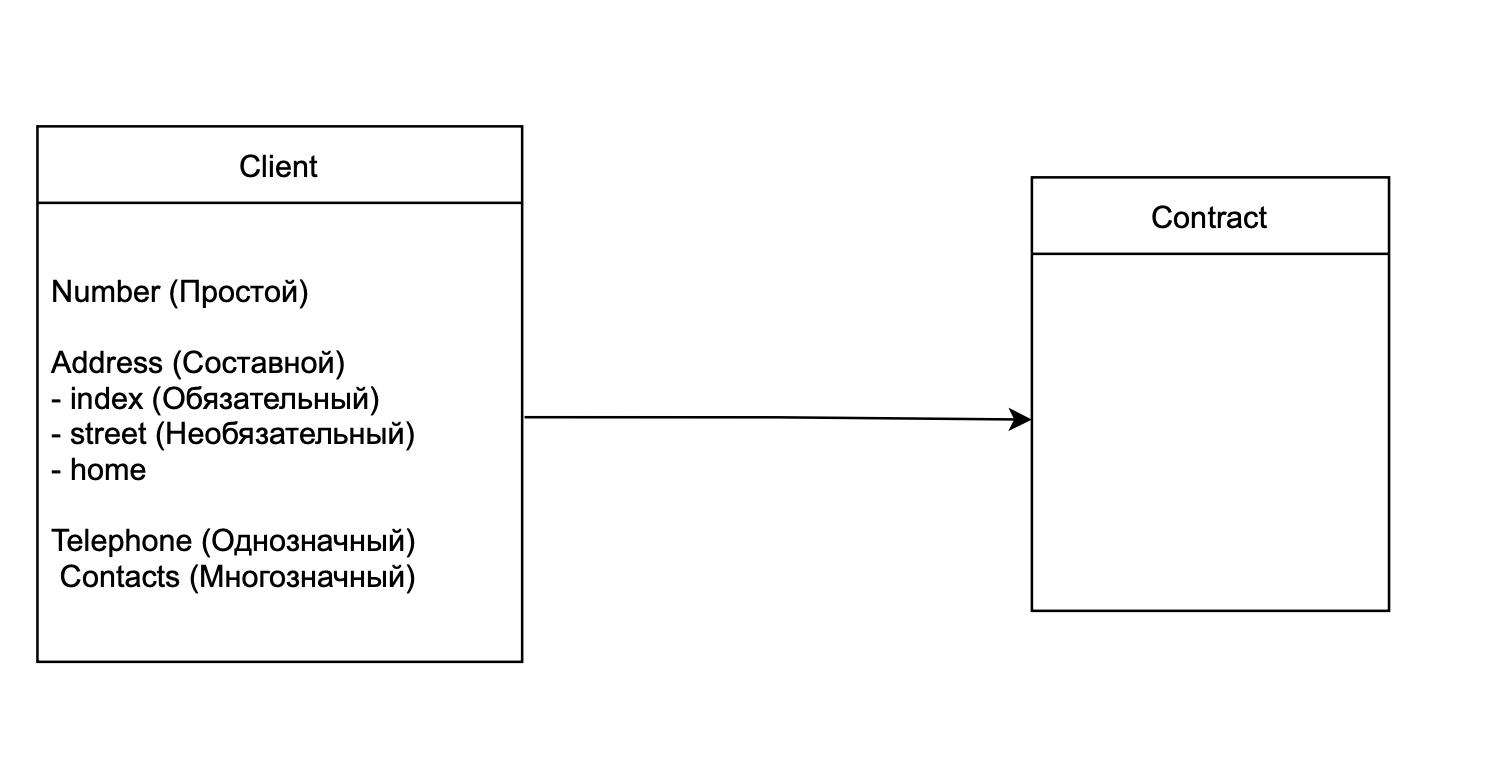
\includegraphics[scale=0.55]{data/client_1.png}

\emph{Атрибуты} -- свойства сущности.

\begin{itemize}
    \item Простые и составные
    \item Обязательные и необязательные
    \item Однозначные и многозначные
\end{itemize}

Типы связей:
\begin{itemize}
    \item Один к одному
    \item Один ко многим
    \item Многие ко многим
\end{itemize}

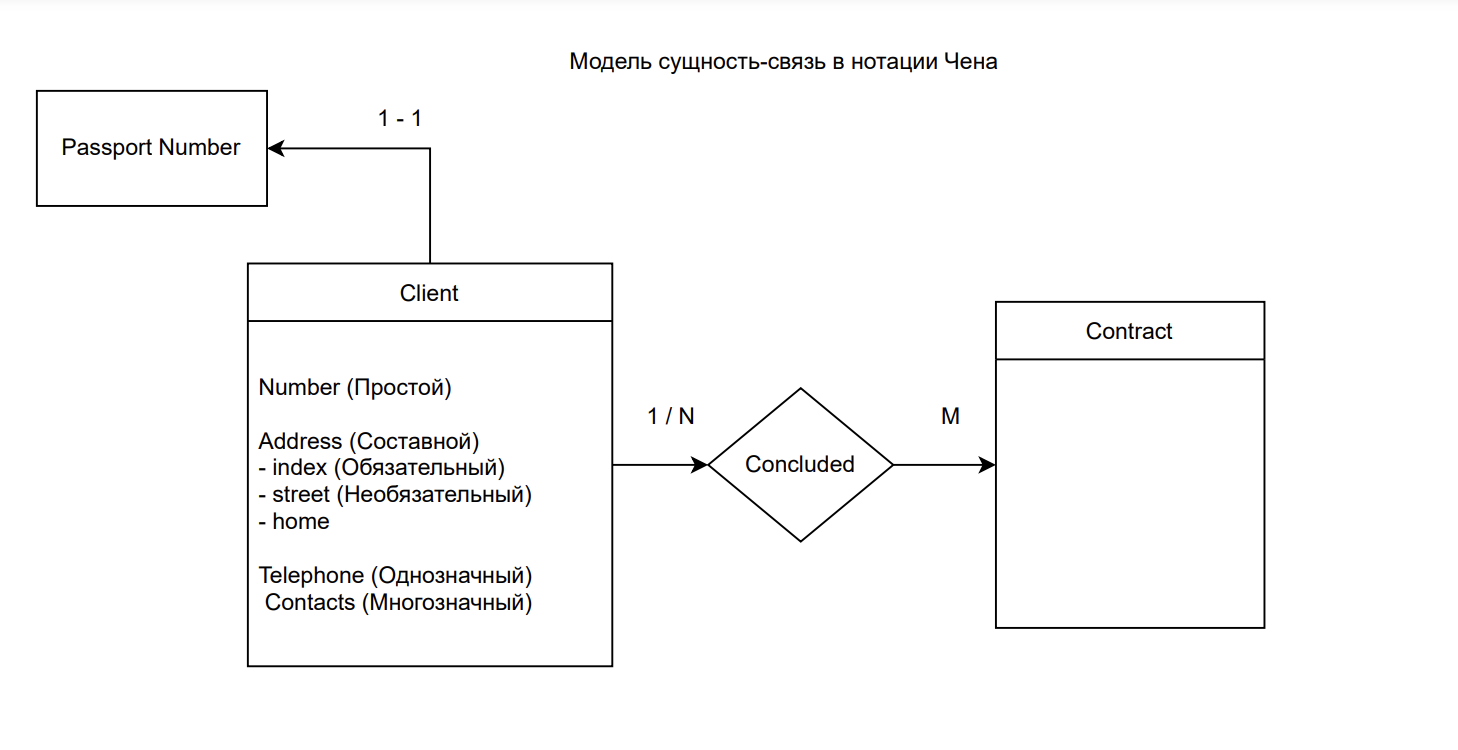
\includegraphics[scale=0.7]{data/client_2.png}

Данная модель универсальна

\subsection{Логическая модель}

\begin{itemize}
    \item Иерархическая
    \item Сетевая
    \item Реляционная
    \item ...
\end{itemize}

Выбор модели зависит от того, какую задачу мы выполняем и как хотим смоделировать данные.

\subsection{Физическая модель}

\begin{itemize}
    \item Определяем ограничения на именование объектов и способы доступа и обращения к ним.
    \item Определяем ограничения на типы данных - определяем домены (множество значений для атрибута).
    \item Описание индексов и их хранение
    \item Вопрос разделения на отдельные файлы
\end{itemize}
\end{document}
